\section{Newtons lover}

Newtons første lov sier at et legeme som ikke er påvirket av noen kraft, eller der summen av kreftene er null, holder seg i ro eller beveger seg med konstant fart langs en rett linje.

\begin{definisjon}[Kraft]
En kraft er en påvirkning som kan endre bevegelsestilstanden til et legeme. Kraft måles i newton, \unit{\newton}.
\end{definisjon}

\begin{formel}[Newtons 2. lov]
\[
  \sum \vec{F} = m\vec{a}
\]
\end{formel}

Tyngdeakselerasjonen er $g = \qty{9.81}{\meter\per\second\squared}$, og tyngden er $G = mg$. Med $m = \qty{2,5}{\kilo\gram}$ får vi $G = \qty{24.5}{\newton}$. Tallet 9,81 skrives også direkte i matematikk: $9,81 \cdot 2,5$.

\subsection{Kraftdiagram på skråplan}

\begin{figure}[H]
\centering
\begin{tikzpicture}[scale=1.1,>={Stealth[length=3mm]}]
  \coordinate (A) at (0,0);
  \coordinate (B) at (5,0);
  \coordinate (C) at (5,2.5);
  \draw[thick] (A) -- (B) -- (C) -- cycle;
  \pic[draw,"$\alpha$",angle eccentricity=1.4,angle radius=9mm] {angle=B--A--C};
  \coordinate (M) at ($(A)!0.55!(C)$);
  \node[draw,fill=gray!20,rotate=26.57,minimum width=1cm,minimum height=0.6cm,anchor=south] (box) at (M) {};
  \draw[->,thick,red] (box.center) -- ++(0,-1.6) node[below] {$G$};
  \draw[->,thick,blue] (box.center) -- ++(116.57:1.4) node[above left] {$N$};
  \draw[->,thick,sngreen] (box.center) -- ++(206.57:1.0) node[left] {$R$};
\end{tikzpicture}
\caption{Kloss på skråplan med vinkel $\alpha$.}
\end{figure}

Komponentene til tyngden:
\begin{align*}
  G_x &= mg\sin\alpha \\
  G_y &= mg\cos\alpha
\end{align*}

\begin{eksempel}[Kloss på skråplan]
En kloss med masse \qty{3.0}{\kilo\gram} ligger på et skråplan med $\alpha = \ang{30}$. Finn akselerasjonen når friksjonen er null.

\begin{losning}
\[
  a = \frac{G_x}{m} = g\sin\alpha = \qty{9.81}{\meter\per\second\squared}\cdot\sin\ang{30} = \qty{4.9}{\meter\per\second\squared}
\]
\end{losning}
\end{eksempel}

\begin{merknad}
I notatet står det $a = g\cos\alpha$ i siste linje, men utregningen over bruker $\sin\alpha$. Det ser ut som en skrivefeil.
\end{merknad}

\subsection{Bevegelse}

Farten er den deriverte av posisjonen: $v = \dv{s}{t}$, og $a = \ddv{s}{t}$. Partielt: $\pdv{U}{x}$. Absoluttverdi $\abs{\vec{v}}$, enhetsvektor $\vu{x}$, vektor $\vb{F}$.

\begin{center}
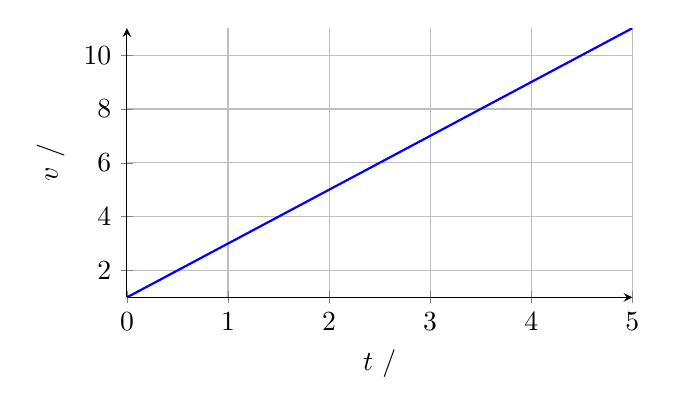
\begin{tikzpicture}
\begin{axis}[width=8cm,height=5cm,xlabel={$t$ / \unit{\second}},ylabel={$v$ / \unit{\meter\per\second}},grid=major,axis lines=left]
\addplot[thick,blue,domain=0:5] {2*x+1};
\end{axis}
\end{tikzpicture}
\end{center}

\begin{husk}
Enheten for akselerasjon er \unit{\meter\per\second\squared}. Ordet \uleselig{akselerasjon} var vanskelig å lese.
\end{husk}

\begin{oppgave}[2.14]
Regn ut strømmen i kretsen.
\end{oppgave}

\begin{center}
\begin{circuitikz}
\draw (0,0) to[battery1, l=$U$] (0,3) to[R, l=$R_1$] (3,3) to[R, l=$R_2$] (3,0) -- (0,0);
\end{circuitikz}
\end{center}

Kjernereaksjon: \ce{^{235}_{92}U + ^{1}_{0}n -> ^{141}_{56}Ba + ^{92}_{36}Kr + 3 ^{1}_{0}n}

\begin{tabular}{@{}lll@{}}
\toprule
Størrelse & Symbol & Enhet \\
\midrule
Masse & $m$ & \unit{\kilo\gram} \\
Kraft & $F$ & \unit{\newton} \\
\bottomrule
\end{tabular}

\begin{itemize}
  \item Første punkt med $\cancel{m}a = \cancel{m}g$.
  \item Andre punkt.
\end{itemize}

\originalfigur[0.5]{fig1}{Skisse fra notatet}

\manglerfigur{tegning av pendel}
